\documentclass[10pt,openright,twoside,french]{book}

\usepackage{marvosym}
\input philippe2013
\input philippe2013_activites

\pagestyle{empty}

\begin{document}

\TitreExo{1}{Opérations sur les nombres\par \'Equations et inéquations}

\exo

Pour chaque nombre de la première colonne, dire s'il appartient ou non aux ensembles proposés. Il ne faut pas répondre au hasard : effectuer alors quelques calculs pour répondre.

\begin{center}
\small
\renewcommand\arraystretch{1.25}
    \begin{tabular}{|c|rl|}
        \hline
            \multirow{5}*{$\frac{462}{385}$} & entier naturel & $\square$ Vrai \quad $\square$ Faux \\
            & entier relatif & $\square$ Vrai \quad $\square$ Faux \\
            & nombre décimal & $\square$ Vrai \quad $\square$ Faux \\
            & nombre rationnel & $\square$ Vrai \quad $\square$ Faux \\
            & nombre réel & $\square$ Vrai \quad $\square$ Faux \\
        \hline
            \multirow{5}*{$\sqrt{147} - 7\sqrt3$} & entier naturel & $\square$ Vrai \quad $\square$ Faux \\
            & entier relatif & $\square$ Vrai \quad $\square$ Faux \\
            & nombre décimal & $\square$ Vrai \quad $\square$ Faux \\
            & nombre rationnel & $\square$ Vrai \quad $\square$ Faux \\
            & nombre réel & $\square$ Vrai \quad $\square$ Faux \\
        \hline
            \multirow{5}*{$\frac{144}{14}$} & entier naturel & $\square$ Vrai \quad $\square$ Faux \\
            & entier relatif & $\square$ Vrai \quad $\square$ Faux \\
            & nombre décimal & $\square$ Vrai \quad $\square$ Faux \\
            & nombre rationnel & $\square$ Vrai \quad $\square$ Faux \\
            & nombre réel & $\square$ Vrai \quad $\square$ Faux \\
        \hline
            \multirow{5}*{$\sqrt{98} - 3\sqrt 2$} & entier naturel & $\square$ Vrai \quad $\square$ Faux \\
            & entier relatif & $\square$ Vrai \quad $\square$ Faux \\
            & nombre décimal & $\square$ Vrai \quad $\square$ Faux \\
            & nombre rationnel & $\square$ Vrai \quad $\square$ Faux \\
            & nombre réel & $\square$ Vrai \quad $\square$ Faux \\
        \hline
    \end{tabular}
\end{center}\[*\]

\exo
On considère l'expression $A(x) = x^2 - \big[2(3-x)\big]^2$.
\begin{enumerate}
    \item Calculer $A(-2)$.
    \item Développer l'expression $A(x)$.
    \item Factoriser $A(x)$.
    \item Résoudre l'équation $A(x) = 0$.
\end{enumerate}\[*\]

\exo
Pour tous nombres réels $a$ et $b$, on considère les deux propositions suivantes :
\[\psframebox{1} \quad (a + b)^2 = 0 \quad\qetq\quad \psframebox{2}\quad a = 0 \text{ et } b = 0.\]

\begin{enumerate}
    \item Expliquer pourquoi $\psframebox 2 \Rightarrow \psframebox 1$.
    \item Est-il vrai que $\psframebox 1 \Rightarrow \psframebox 2$ ? Justifier.
    \item Est-il vrai que $\psframebox 1 \Leftrightarrow \psframebox 2$ ? Justifier.
    \item Trouver deux propositions simples \psframebox{$3$} et $\psframebox 4$ telles que $\psframebox 3 \Leftrightarrow \psframebox 4$.
\end{enumerate}\[*\]\clearpage

\exo
On considère l'expression $B(x) = x^2 + 4x + 4 - 9(x^2 - 4)$.\par
Combien de solutions dans $\N$ admet l'équation $B(x) = 0$ ? Et dans $\Z$ ?\[*\]

\exo
Résoudre dans $\R$ les inéquations suivantes :
\[x+ 4 > 2 \qq -2x + 6 \geq 8 \qq -\frac{5x}{2} + \frac4 3 \leq -\frac x 3 + \frac 7 2\]\[*\]

\exo
On considère les intervalles suivants :
$A = \intervalleof{-\infty}{3} \qq B = \intervalleof{-2}{6} \qq C = \intervalleff 0 3 \qetq D = \intervallefo{3}{+\infty}.$
\begin{enumerate}
    \item Traduire par des égalités les quatre intervalles ci-dessus.
    \item Déterminer les intervalles suivants :
    \[A \cap B \qq A \cup B \qq B \cap C \qq B \cup C \qq A \cap D \qq A \cup D\]
\end{enumerate}\[*\]

\exo
Les propositions suivantes sont-elles vraies ? Justifier les réponses. Si elles sont vraies, les écrire sous la forme $A \Rightarrow B$.
\begin{enumerate}
    \item Si $a \in \intervalleff{-1}{3}$ alors $a \geq -1$.
    \item Si $b \geq -1$ alors $b \in \intervalleff{-1}{3}$.
    \item Si $c < 2$ et $d < -3$ alors $c \times d < -6$.
    \item Si $e > 2$ et $f > 3$ alors $e \times f > 6$.
\end{enumerate}\[*\]

\exo
$ABCD$ est un carré de côté $10~cm$ et le point $F$ est placé sur le segment $[CD]$ de telle façon que $FC = 3~cm$.\par
$E$ est un point quelconque du segment $[BC]$ et on pose, en centimètres, $CE = x$.

\begin{center}
    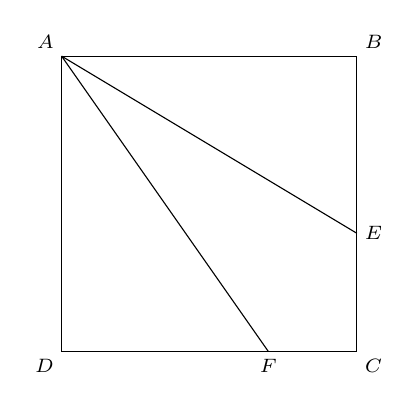
\begin{tikzpicture}[scale=0.75]
        \coordinate (A) at (0,5); \coordinate (B) at (5,5); \coordinate (C) at (5,0); \coordinate (D) at (0,0);
        \draw (A) -- (B) -- (C) -- (D) -- cycle;
        \coordinate (E) at (5,2); \coordinate (F) at (3.5,0);
        \draw (A) -- (E); \draw (A) -- (F);
        \begin{scriptsize}
            \draw (A) node[above left] {$A$}; \draw (B) node[above right] {$B$}; \draw[below right] (C) node {$C$};
            \draw (D) node[below left] {$D$}; \draw[right] (E) node {$E$}; \draw (F) node[below] {$F$};
        \end{scriptsize}
    \end{tikzpicture}
\end{center}

\begin{enumerate}
    \item À quel intervalle appartient $x$ ?
    \item Calculer $AF^2$.
    \item Exprimer $FE^2$ en fonction de $x$.
    \item Montrer que $AE^2 = x^2 - 20x + 200$.
    \item Déterminer la valeur de $x$ pour laquelle le triangle $AFE$ est rectangle en $F$.
\end{enumerate}\[*\]

\exo
On considère un cercle de rayon $\sqrt 7$. On donne les encadrements suivants à $10^{-3}$ près :
\[3{,}141 \leq \pi \leq 3{,}142 \qetq 2{,}645 \leq \sqrt7 \leq 2{,}646.\]
\begin{enumerate}
    \item Donner un encadrement du périmètre $\mtc P$ du cercle à $10^{-1}$ près.
    \item Donner un encadrement de l'aire $\mtc A$ du cercle à $10^{-1}$ près.
\end{enumerate}\[***\]

\end{document} 